%% Bilder f�r PICblock

%\newcommand{\TikZIntegrator}{
%\begin{tikzpicture}
	% Koordinatensystem
%	\draw[thin] (-7\mm,-5\mm) -- (7\mm,5\mm);
%\end{tikzpicture}


\newcommand{\TikZGain}{
\begin{tikzpicture}
		\draw (0,5\mm) -- (14\mm,5\mm);
		\draw[white] (0,0) -- (14\mm,0);
\end{tikzpicture}
}

\newcommand{\TikZsgn}{
\begin{tikzpicture}
	% Koordinatensystem
	\draw[->, very thin] (-4\mm,0) -- (4\mm,0);
	\draw[->, very thin] (0,-4\mm) -- (0,4\mm);
	
	% Signumfunktion
	\draw[thin] (-4\mm,-2\mm) -- (0,-2\mm);
	\draw[thin] (0,-2\mm) -- (0,2\mm);
	\draw[thin] (0,2\mm) -- (4\mm,2\mm);
\end{tikzpicture}
}

\newcommand{\TikZdeadzone}{
\begin{tikzpicture}
	% Koordinatensystem
	\draw[->, very thin] (-4\mm,0) -- (4\mm,0);
	\draw[->, very thin] (0,-4\mm) -- (0,4\mm);
	
	% Deadzone
	\draw[thin] (-3\mm,-4\mm) -- (-2\mm,0);
	\draw[thin] (-2\mm,0) -- (2\mm,0);
	\draw[thin] (2\mm,0) -- (3\mm,4\mm);
\end{tikzpicture}
}

\newcommand{\TikZsaturation}{
\begin{tikzpicture}
	% Koordinatensystem
	\draw[->, very thin] (-4\mm,0) -- (4\mm,0);
	\draw[->, very thin] (0,-4\mm) -- (0,4\mm);

	% Saturation
	\draw[thin] (-4\mm,-2.5\mm) -- (-1\mm,-2.5\mm);
	\draw[thin] (-1\mm,-2.5\mm) -- ( 1\mm, 2.5\mm);
	\draw[thin] ( 1\mm, 2.5\mm) -- ( 4\mm, 2.5\mm);
\end{tikzpicture}
}

%% sonstige Bilder
\newcommand{\TikZRarrow}[1][]{%
\begin{tikzpicture}
	\draw[<-,opacity=0] (-3.8\mm,0) -- (0,0) node[pos=0, anchor=south east, xshift=2\mm, yshift=1\mm] {#1};	% keine Ahnung warum, aber nur mit -3.8 wirds mittig....
	\draw[|->] (0,0) --  node[pos=1, anchor=south west, xshift=-2\mm, yshift=1\mm] {#1} (5\mm,0);
\end{tikzpicture}%
}

\newcommand{\TikZspring}[1][10]{%
\begin{tikzpicture}
	\foreach \x in{0,1,...,3}
		\draw[thick, line join=round, line cap=round] (#1*0.25*\x\mm,0) -- (#1*0.0625\mm+#1*0.25*\x\mm,2\mm) -- (#1*0.1875\mm+#1*0.25*\x\mm,-2\mm) -- (#1*0.25\mm+#1*0.25*\x\mm,0\mm);
	\draw[thick] (0,0) -- ++(-1\mm,0);
	\draw[thick] (#1\mm,0) -- ++(1\mm,0);
\end{tikzpicture}%
}

\newcommand{\TikZdamper}{%
\begin{tikzpicture}
	\draw[thick] (0,0) -- (2\mm,0);
	\draw[thick] (2\mm,1\mm) -- (2\mm,-1\mm);
	\draw[thick] (1\mm,1.5\mm) -- (3\mm,1.5\mm) -- (3\mm,-1.5\mm) -- (1\mm,-1.5\mm);
	\draw[thick] (3\mm,0) -- (5\mm,0);
\end{tikzpicture}%
}


\newcommand{\TikZrwall}{%
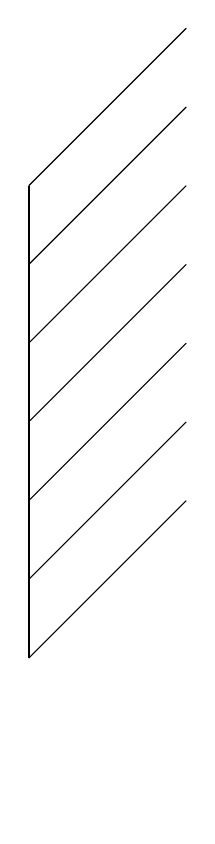
\begin{tikzpicture}
\draw[thick] (0,0\mm) -- (0,6\mm);
\draw[white] (0,0\mm) -- (0,-2\mm); % Damit der Block zentriert ist (unsch�ne L�sung...)
\foreach \x in{0,1,...,6}
	\draw (0,\x\mm) -- ++(2\mm,2\mm);
\end{tikzpicture}%
}

\newcommand{\TikZlwall}{%
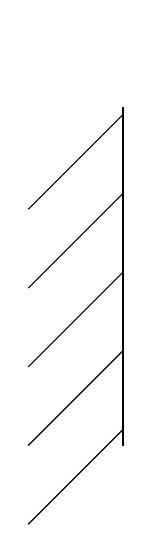
\begin{tikzpicture}
	\draw[thick] (0,-0.2\mm) -- (0,4.1\mm);
	\foreach \x in{0,1,...,4}
		\draw (0,\x\mm) -- ++(-1.2\mm,-1.2\mm);
	\draw[opacity=0] (0,4.1\mm) -- (0,5.1\mm); % Damit der Block zentriert ist (unsch�ne L�sung...)
\end{tikzpicture}%
}